\section{Durchführung}
\label{sec:Durchführung}
Es wird das Elastizitätsmodul $E$ zweier Stäbe ermittelt.
Diese unterscheiden sich im Material und im Querschnitt $Q$.
Der erste Stab hat einen runden Querschnitt, der zweite einen quadratischen.
Die einseitige Spannung soll mit beiden Stäben durchgeführt werden.
Bei der beidsseitigen Einspannung wird einer der beiden Stäbe ausgewählt.
\begin{figure}
    \centering
    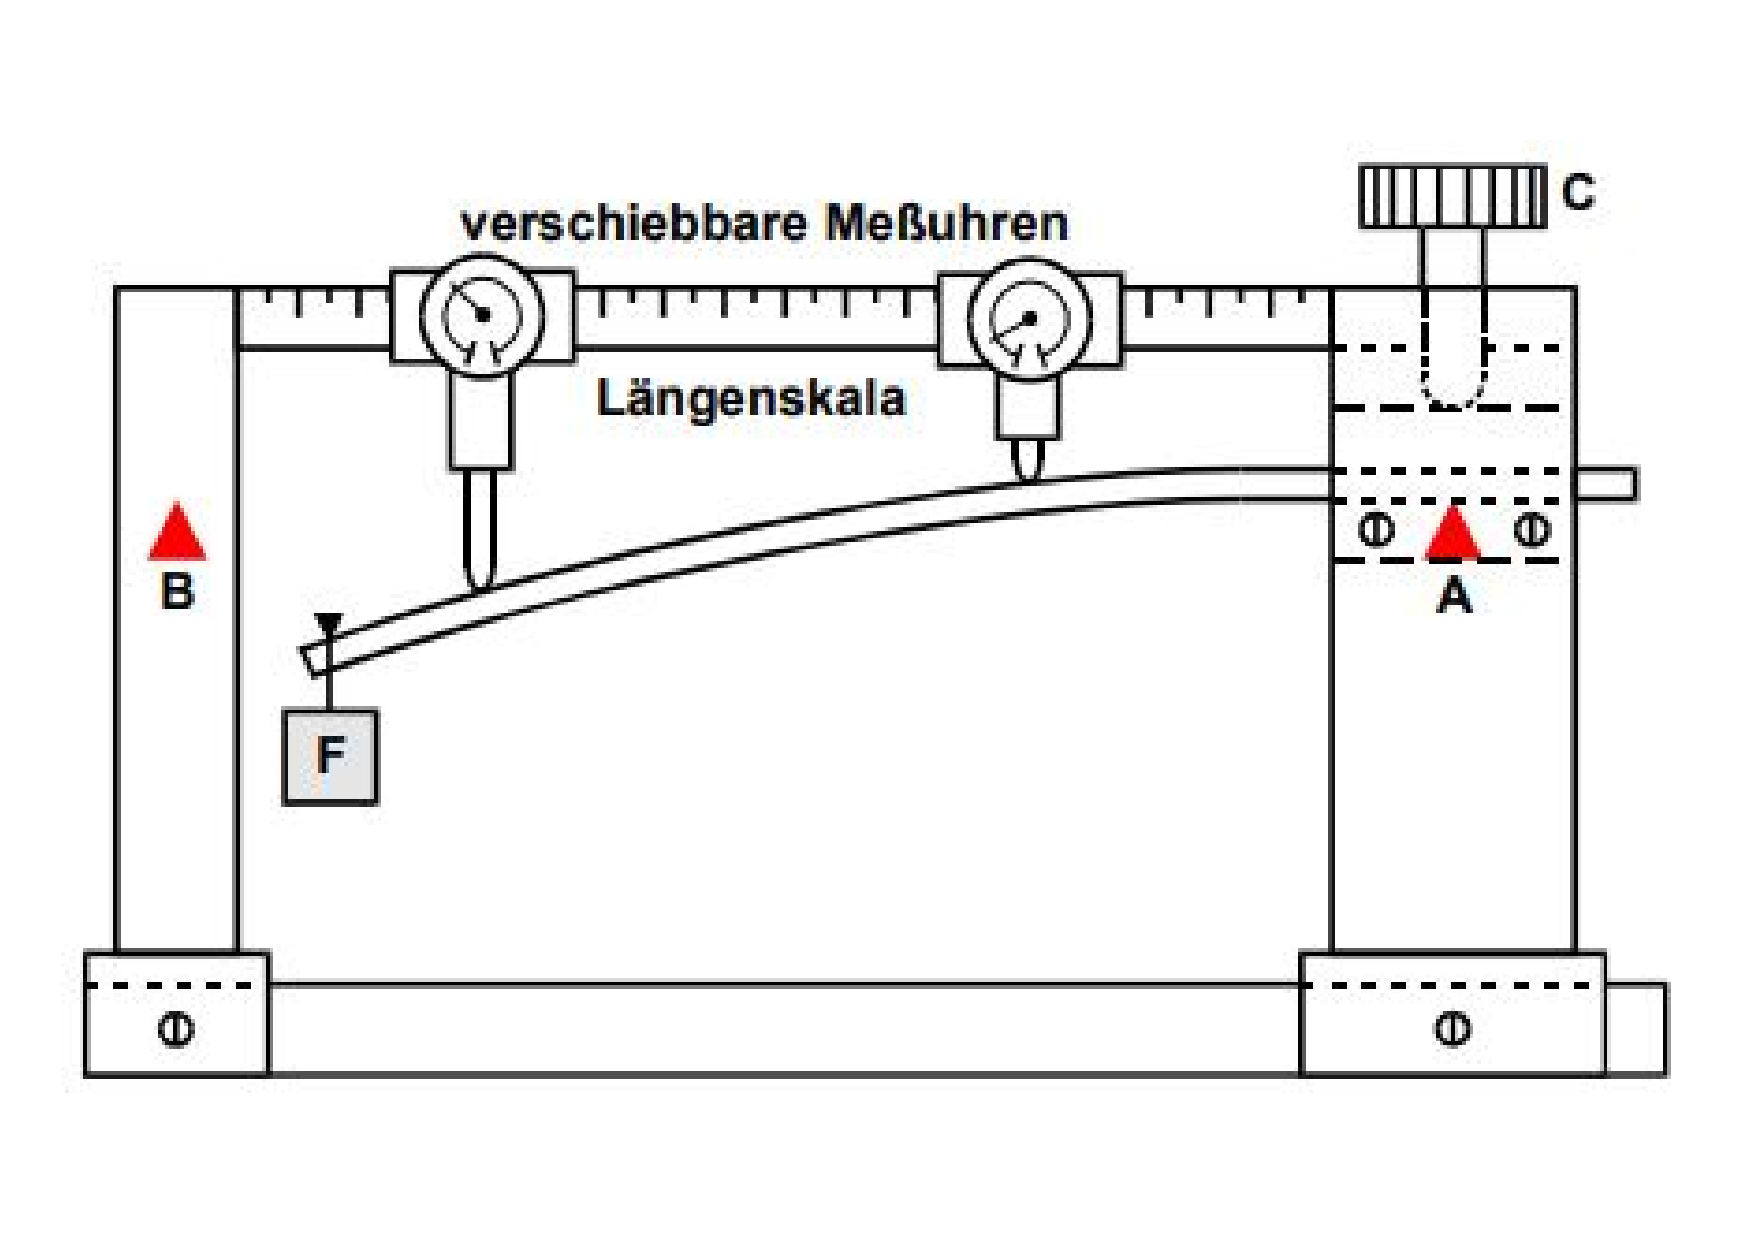
\includegraphics[width=\textwidth]{Messapparat.pdf} 
    \caption{Schematischer Aufbau der Apparatur zur Vermessung der elastisch gebogenen Stäbe aus \cite{anleitung}.}
    \label{fig:Messapparat}
\end{figure}
\subsection{Einseitige Einspannung}
\label{subsec:einseitigeEinspannung}
Der Stab soll wie in Abbildung \ref{fig:Messapparat} eingespannt werden.
An dem freien Ende greift eine Kraft $F$ an, die den Stab biegt.
Da die Stäbe nicht vollkommen gerade sind, wird zuvor eine Nullmessung durchgeführt.
Dabei wird in regelmäßigen Abständen $x$ mithilfe von Messuhren die Durchbiegung $D_0$ ohne angreifende Kraft gemessen.
Es wird an 20 Stellen gemessen.
Danach wird das Gewicht an das freie Ende des Stabes gehängt und an den gleichen Stellen $x$ die Durchbiegung $D_M$ gemessen.
Die Differenz von $D_M(x)$ und $D_0(x)$ ist dann die tatsächliche Durchbiegung $D(x)$.

Für beide Stäbe wird jeweils das angehängte Gewicht $m$ gewogen, die Länge $L$ und die Breite/ der Durchmesser $d$ mithilfe eines Messbandes und der Schieblehre gemessen.
Bei der Länge des Stabes wird nur der Teil vom freien Ende bis zur Einspannung in Betracht gezogen.
Dabei wird die Messung der Eigenschaften der Stäbe fünf Mal wiederholt.

\subsection{Beidseitige Einspannung}
Für die beidseitige Einspannung wird der Stab mit dem runden Querschnitt gewählt.
Seine Enden werden an den Punkten A und B eingespannt (Abbildung \ref{fig:Messapparat}).
Auch hier wird zuvor eine Nullmessung durchgeführt.
Auf beiden Hälften werden an jeweils 7 Stellen mit regelmäßigen Abstand Messungen vorgenommen.
Daraufhin wird an die Mitte des Stabes das Gewicht gehängt und erneut die Durchbiegung an den gleichen Stellen $x$ gemessen.
Die tatsächliche Durchbiegung $D(x)$ wird wie in \ref{subsec:einseitigeEinspannung} ermittelt.

Das angehängte Gewicht $m$ wird gewogen und der Abstand zum Aufhängepunkt gemessen.

\begin{figure}
    \centering
    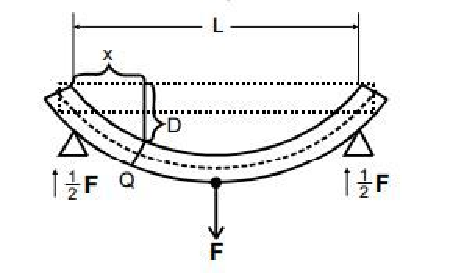
\includegraphics[width=\textwidth]{zweiseitig.pdf}
    \caption{Durchbiegung eines Stabes bei zweiseitiger Einspannung nach \cite{anleitung}.} 
\end{figure}